% sets, dictionaries(no time left in lecture5)
% file I/O, exceptions, debugging
% created by Uwe Schadewald
% modified by Mathias Kuntze and Ahmet Uysal
% Add, handout to documentclass arguments for condensed pdf
\documentclass[presentation, 8pt, mathserif, t]{beamer} % , aspectratio=169
\usepackage[english]{babel}
\usepackage{pgf,graphicx}
\usepackage{amsmath, amssymb}
\usepackage[utf8]{inputenc}
\usepackage{lmodern}
\usepackage{palatino}
\usepackage{multimedia}
\usepackage{pgfpages} 
\usepackage{tikz}
\usepackage{datetime}
\pdfoptionpdfminorversion=5

\usepackage{caption}
\usepackage{subcaption}
% if else
\usepackage{ifthen}
% extend table options
\usepackage{tabularx} 
\usepackage{booktabs}
\usepackage{multicol}
\usepackage{multirow}
\usepackage{eso-pic}  % package to set background image
\usepackage[calc]{picture}

% Packages and stuff for ToDo list like itempoints
\usepackage{pifont}
\newcommand{\cmark}{\ding{51}}%
\newcommand{\xmark}{\ding{55}}%
\newcommand{\open}{$\square$}
\newcommand{\done}{\rlap{$\square$}{\raisebox{1pt}{\large\hspace{1.5pt}\cmark}}\hspace{-2.5pt}}
\newcommand{\wontfix}{\rlap{$\square$}{\raisebox{1pt}{\large\hspace{1.5pt}\xmark}}}
\newcommand{\notsure}{\rlap{$\square$}{\raisebox{0.8pt}{\large\hspace{1.5pt}\textbf{?}}}}



% side bar and footer
\setbeamertemplate{headline}{	
	\leavevmode
	\vspace{-4em}	
	\hbox{		
		\begin{beamercolorbox}[wd=0.85\paperwidth,ht=10ex,dp=8ex,center]{}%			
			% navigation with subsections as dots
			\hspace{3.5em}\insertnavigation{0.7\paperwidth}{\hskip0pt plus1fill} % add navigation in footer						
			% navigation with sections, no subsections
			% \insertsectionnavigationhorizontal{0.6\paperwidth}{\hskip0pt plus1fill}{} \\ % add navigation in footer}
			
		\end{beamercolorbox} 				
	}
	\vskip0pt
}


\setbeamertemplate{footline}{	
	\leavevmode
	\vspace{-3em}
	\hbox{
		\begin{beamercolorbox}[wd=.33\paperwidth,ht=2.25ex,dp=1ex,left]{author in head/foot}%
			\hspace{5em}
			\insertshortauthor
		\end{beamercolorbox}
		\begin{beamercolorbox}[wd=.33\paperwidth,ht=2.25ex,dp=1ex,center]{title in head/foot}%
			\insertshorttitle \ - \insertshortsubtitle
		\end{beamercolorbox}	
		\begin{beamercolorbox}[wd=0.30\paperwidth,ht=10ex,dp=8ex,right]{pagenumber in head/foot}			 	
			\insertframenumber % add page numbers
		\end{beamercolorbox}
	}			
	\vskip0pt
}



\setbeamertemplate{frametitle}{
	\ifthenelse{\equal{\insertframesubtitle}{}}{
		\vspace{0.6cm}
		\huge{\insertframetitle}
	}{
		\vspace{0.6cm}
		\small{\insertframetitle}\\
		\vspace{0.3cm}
		\huge{\insertframesubtitle}
    }		
}

	
% enumerate sections
\setbeamertemplate{section in head/foot}{\hfill\insertsectionheadnumber.~\insertsectionhead}
%\setbeamertemplate{section in head/foot shaded}{\color{structure!50}\hfill\insertsectionheadnumber.~\insertsectionhead}
\setbeamertemplate{section in toc}{\inserttocsectionnumber.~\inserttocsection}

%enumerate subsections
\setbeamertemplate{subsection in head/foot}{\hfill\insertsubsectionheadnumber.~\insertsubsectionhead}
\setbeamertemplate{subsection in head/foot shaded}{\color{structure!50}\hfill\insertsubsectionheadnumber.~\insertsubsectionhead}
%\setbeamertemplate{subsection in toc}[subsections numbered]
\setbeamertemplate{subsection in toc}{\vskip0.5em\leftskip=2em\inserttocsubsection\par}

%--------------------------Common------------------------------------------------------
\setbeamercovered{transparent} % make the beamer theme invisible
\usefonttheme{structurebold}
\beamertemplatenavigationsymbolsempty % set navigations helper function to off
\setbeamertemplate{bibliography item}[text]
\setbeamertemplate{note page}[plain]

%\setlist[itemize,1]{label={$\bullet$}} % \item are using bullets
\setbeamertemplate{itemize items}[circle]
	
	

	
% create a new command to show it on two screens
% I'm using dspdfviewer.
\newcommand{\setDualView} {
	\setbeameroption{show notes on second screen=right}
}

%\AtBeginSection[]{\subsection{}}
\newcommand{\addcite}[1]{%
	\AddToShipoutPictureFG*{%
		\AtPageLowerLeft{%
			\put(0.90\paperwidth,5em){											
				\tiny{
					\cite{#1} 
				}			
			}
		}
	}	
}

% insert a frame with references -> use bibtex
\newcommand{\insertReferenceFrame}[3]{%
	\section{#1}
	\begin{frame}[allowframebreaks]
		\frametitle{#1}
		\bibliographystyle{#2}
		\bibliography{#3}
	\end{frame}	
}

\AtBeginSection[]{\subsection{}}
	





\usepackage{../KU-Beamer-Template/style/koc} 
\usepackage{minted}
\usepackage{upquote}
\usepackage{graphicx}
\usepackage{tikz}
\usetikzlibrary{shapes.symbols,positioning, chains}

\title{KOLT Python}
\subtitle{File I/O, Testing \& Debugging} 
\newdate{date}{25}{03}{2019}
\date{\displaydate{date}}
\author{Ahmet Uysal}

\titlegraphic{
\includegraphics[scale=0.2]{../KU-Beamer-Template/style/images/logo_kolt.eps}}

\setbeamercovered{invisible} % transparent

\begin{document}
    \maketitle

    \frame{\frametitle{Agenda}\tableofcontents}

    \section{Recap}

    \begin{frame}{Mutability}
        \huge
        \textbf{Immutable:}\\
        \LARGE
        An \texttt{\textbf{object}} with a fixed value.
         Immutable objects include \textbf{numbers}, \textbf{strings} and \textbf{tuples}. Such an object cannot be altered.
         A new object has to be created if a different value has to be stored.
         They play an important role in places where a constant \textbf{hash value} is needed, for example as a \textbf{key} in a \texttt{dictionary}.
        \inputminted[frame=single,framesep=2pt]{python3}{../Lecture5/code-examples/value_update.py}
    \end{frame}

    \begin{frame}{Python Data Model}
        \LARGE
        How did we represent data in Python?
         \textbf{Variables!}\\
        How do they work?
         Do they store the data themselves?
        \begin{columns}
            \begin{column}{0.5\textwidth}
                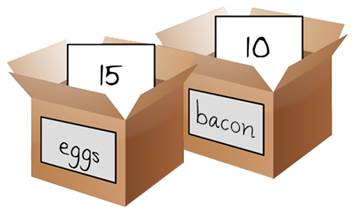
\includegraphics[width=0.9\textwidth]{../Lecture5/images/box.jpg}
            \end{column}
            \begin{column}{0.5\textwidth}
                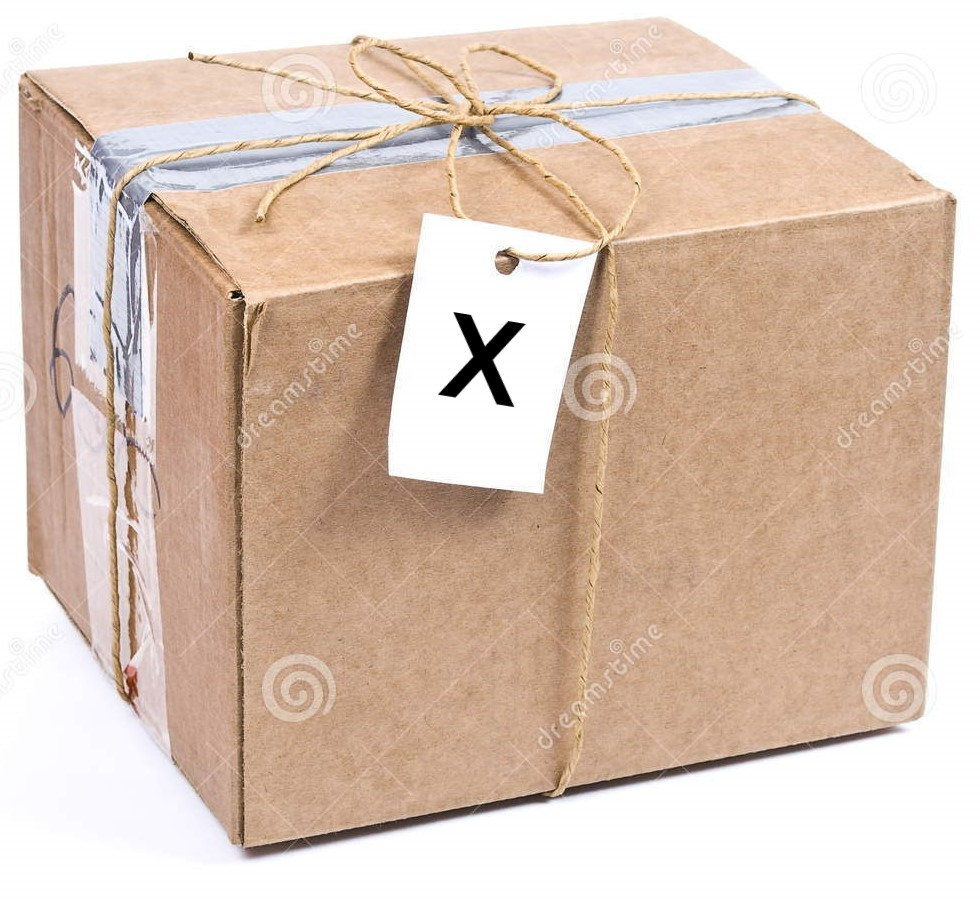
\includegraphics[width=0.6\textwidth]{../Lecture5/images/box_tag.jpg}
            \end{column}
        \end{columns}
    \end{frame}

    \begin{frame}{Box Analogy}
        \LARGE
        \inputminted[frame=single,framesep=2pt,lastline=4]{python3}{../Lecture5/code-examples/box_counter_ex.py}
        \inputminted[frame=single,framesep=2pt,firstline=6]{python3}{../Lecture5/code-examples/box_counter_ex.py}
        Did we just changed inside of a closed box?
         Box analogy \textbf{does not} work!
    \end{frame}

    \begin{frame}{Python Data Model}
       \begin{columns}
            \begin{column}[c]{0.5\textwidth}
                \LARGE
                \texttt{my\_secret\_box = [0, 1, 2]}\\
                \visible<5->{\texttt{other\_box = my\_secret\_box}\\}
                \visible<8->{\texttt{other\_box.remove(2)}\\}
                \visible<10->{\texttt{print(my\_secret\_box)}}
            \end{column}
            \begin{column}[c]{0.5\textwidth}
                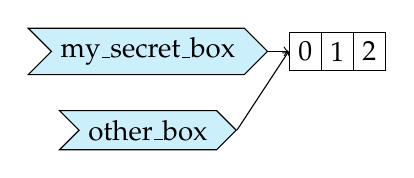
\begin{tikzpicture}%[node distance=-0.15mm]
                    \visible<3->{\node[signal, draw, signal from=west, fill=cyan!20] (var1) {my\_secret\_box};}
                    \visible<2->{
                        \begin{scope}[start chain, right of= var1, node distance=-.5pt, shift={(1,0)}]
                            \def\index{2}
                            \foreach \x in {0,1,2} {
                                \ifx\x\index
                                \visible<2-8>{\node [draw,on chain] (arr\x) {\x};}
                                \else
                                \node [draw,on chain] (arr\x) {\x};
                                \fi
                            } 
                        \end{scope}
                    }
                    \visible<4->{\draw[->] (var1.east) -- (arr0.west);}
                    \visible<6->{\node[signal, draw, signal from=west, fill=cyan!20, below of=var1] (var2) {other\_box};}
                    \visible<7->{\draw[->] (var2.east) -- (arr0.west);}
                \end{tikzpicture}
           \end{column}
       \end{columns}
       \bigskip
       \LARGE
       \visible<11->{Variables are more like \textbf{labels} pointing to \textbf{values}!\\}
       \visible<12->{\textbf{Assignment} links \textbf{variables} to \textbf{values}!}
    \end{frame}


    \begin{frame}{Mutability}
        \huge
        \textbf{Immutable:}\\
        \LARGE
        An \texttt{\textbf{object}} with a fixed value.
        %\pause
         Immutable objects include \textbf{numbers}, \textbf{strings} and \textbf{tuples}. Such an object cannot be altered.
        %\pause
         A new object has to be created if a different value has to be stored.
        %\pause
         They play an important role in places where a constant \textbf{hash value} is needed, for example as a \textbf{key} in a \texttt{dictionary}.
        %\pause
        \inputminted[frame=single,framesep=2pt]{python3}{../Lecture5/code-examples/value_update.py}
    \end{frame}

    \begin{frame}{Object}
        \LARGE
        \textbf{Everything} is an object in Python.
         Even though variables \textbf{do not} have \texttt{types}, each object has a \textbf{fixed} \texttt{type}.\\
        $\hookrightarrow$ Values at the right side of our label analogy are objects!
        \bigskip
        \begin{columns}
            \begin{column}[c]{0.5\textwidth}
                \LARGE
                \visible<2->{\texttt{a = 5}\\}
                \visible<6->{\texttt{a = 10}\\}
                \visible<10->{\texttt{a += 3}\\}
                \visible<14->{\texttt{print(a)}}
            \end{column}
            \begin{column}[c]{0.5\textwidth}
                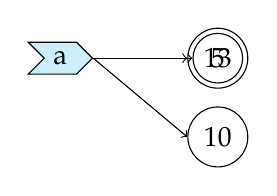
\begin{tikzpicture}%[node distance=-0.15mm]
                    \visible<4->{\node[signal, draw, signal from=west, fill=cyan!20] (var1) {a};}
                    \visible<3-8>{\node[circle, draw, right of=var1, shift={(1,0)}] (val1) {5};}
                    \visible<5-7>{\draw[->] (var1.east) -- (val1.west);}
                    \visible<7-12>{\node[circle, draw, below of=val1] (val2) {10};}
                    \visible<8-11>{\draw[->] (var1.east) -- (val2.west);}
                    \visible<11->{\node[circle, draw, right of=var1, shift={(1,0)}] (val3) {13};}
                    \visible<12->{\draw[->] (var1.east) -- (val3.west);}
                \end{tikzpicture}
           \end{column}
       \end{columns}
    \end{frame}

    \begin{frame}{Object}
        \LARGE
        Each object has an \texttt{identity},
         this value can be obtained by using \texttt{\textbf{id()}} function.\\
        \textbf{==} operator compares values, \textbf{\texttt{is}} operator compares identities. 
        \inputminted[frame=single,framesep=2pt]{python3}{../Lecture5/code-examples/identity.py}
        Almost always use \textbf{==} to compare values!
    \end{frame}

    \begin{frame}{Aliasing \& Cloning}
        \Large
        \begin{columns}
            \begin{column}[c]{0.6\textwidth}
                \begin{itemize}
                    \item More than one variables can refer to \textbf{same object}!
                    \item What if we want to clone/copy instead of aliasing?
                    \item For lists, \texttt{list.copy()} $\Rightarrow$ returns a \underline{shallow copy} of the list.
                    \item Shallow: only copy the references, not inner values.
                    \item \texttt{>>> import copy}
                \end{itemize}
            \end{column}
            \begin{column}[c]{0.4\textwidth}
                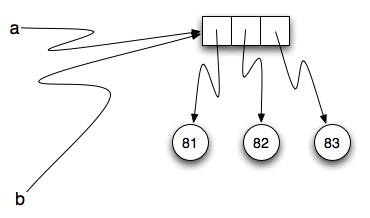
\includegraphics[width=0.9\textwidth]{../Lecture5/images/aliasing.png}
            \end{column}
        \end{columns}
        \texttt{copy.copy(x)}: shallow copy, \texttt{copy.deepcopy(x)}: deepcopy   
    \end{frame}


    \begin{frame}{Tuples}
        \LARGE
        \begin{itemize}
            \item \textbf{Immutable} sequence(ordered) of elements.
            \item Similar to \texttt{list}s, you can use \textbf{indexing}, \textbf{slicing}, and iterate over using \texttt{for} loops.
            \item Elements cannot be added/removed/changed once the tuple is created.
            \item How to create tuples?
             \textbf{\texttt{my\_tuple = (1, [1, 2], \textquotesingle a\textquotesingle )}}
            \item \textbf{\texttt{len(my\_tuple)}} $\Rightarrow$
             3
            \item \textbf{\texttt{my\_tuple.append(3)}} $\Rightarrow$
             \textbf{\texttt{AttributeError:}} \texttt{\textquotesingle tuple\textquotesingle \ object has no attribute \textquotesingle append\textquotesingle}
        \end{itemize}
    \end{frame}

    \begin{frame}{Tuples}
        \LARGE
        \texttt{() / tuple()}: empty tuple, 
         \texttt{(3)}:
         \texttt{int} 3,
         \texttt{(3,)}:
         \texttt{tuple} containing 3
        \inputminted[frame=single,framesep=2pt]{python3}{../Lecture5/code-examples/tuples.py}
    \end{frame}

    \section{Sets}
    \begin{frame}{Sets}
        \LARGE
        \begin{itemize}
            \item \textbf{Unordered} \underline{sequence} of \textbf{unique} elements.
            \pause
            \item \underline{\textbf{Cannot}} use \textbf{indexing/slicing}, \textbf{can} iterate with \texttt{for} loops.
            \pause
            \item \textbf{Mutable}, \texttt{add(element)}, \texttt{remove(element)} methods.
            \pause
            \item Python also has \textbf{immutable} sets: \texttt{frozenset}
            \pause
            \item How to create sets? 
            \pause
             \texttt{my\_set = \{1, 2, 3, 4, 2\}}
            \item How to create empty sets?
            \pause
             \texttt{set()} (\{\ \} is reserved for \texttt{dict})
            \pause
            \item Can compute set operations: \textbf{union}, \textbf{intersection}, \textbf{difference}, \textbf{symmetric difference}.
        \end{itemize}
    \end{frame}
    \begin{frame}{Sets}
        \centering
        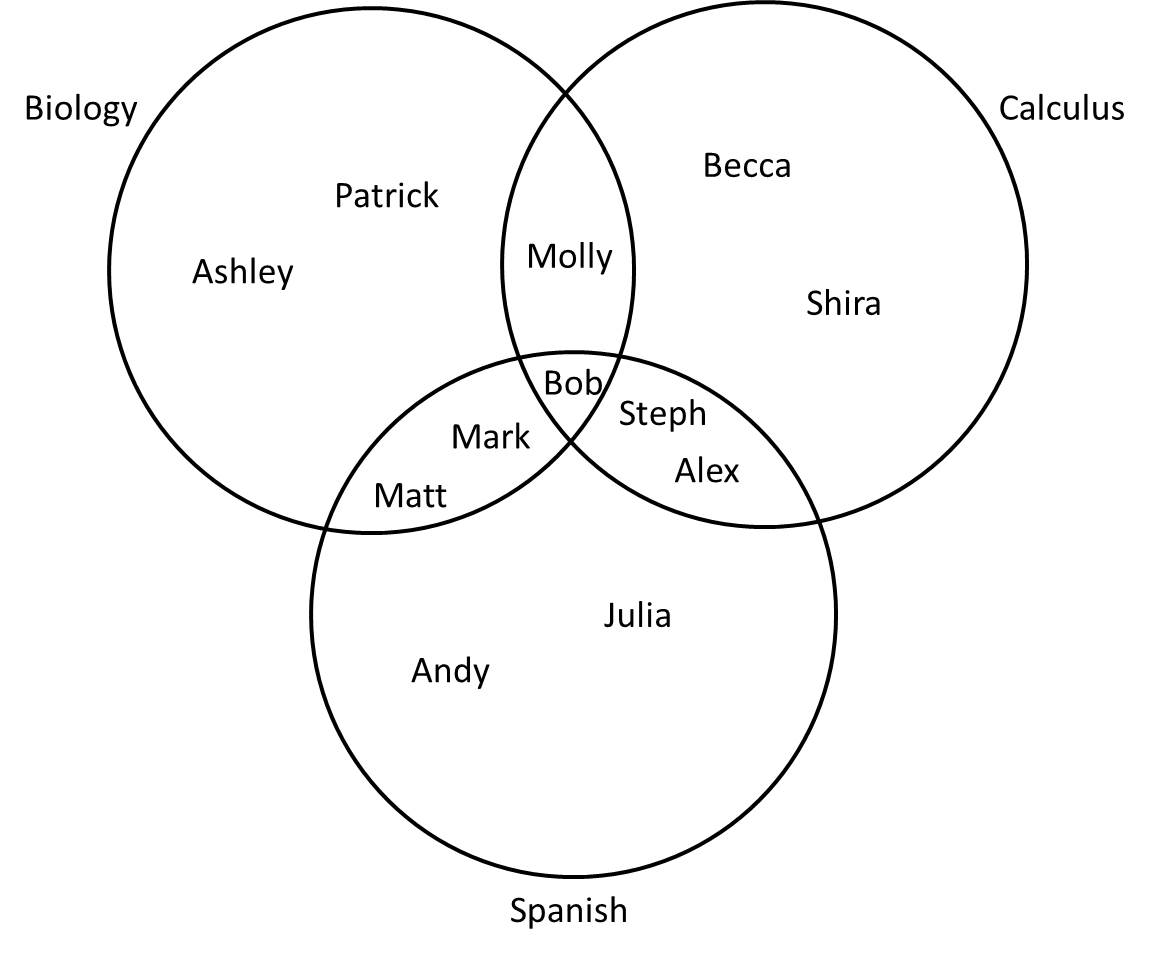
\includegraphics[height=0.75\textheight]{../Lecture5/images/venn.jpg}
    \end{frame}
    \begin{frame}{Sets}
        \inputminted[frame=single,framesep=2pt]{python3}{../Lecture5/code-examples/sets.py}
    \end{frame}
    \section{Dictionaries}
    \begin{frame}{Dictionaries}
        \LARGE
        \begin{itemize}
            \item Collection of \textbf{key$-$value} \underline{pairs}.
            \pause
            \item \underline{\textbf{Cannot}} use \textbf{indexing/slicing}, \textbf{can} iterate with \texttt{for} loops. 
            \pause
            \item In general, they are not \textbf{ordered}. 
            \pause
            \item However, in Python 3.7 pairs are guaranteed to be in insertion order.
            \pause
            \item In other words, we will get pairs in insertion order if we loop over the \texttt{dict}.
            \pause
            \item How to create dictionaries?
            \pause
             \texttt{\{\ \}/dict()}: empty dictionary
            \pause
            \item \texttt{d = \{\textquotesingle one\textquotesingle : 1, \textquotesingle two\textquotesingle : 2, \textquotesingle three\textquotesingle : 3, \textquotesingle four\textquotesingle : 4\}}
            \pause
            \item How to access values? 
            \pause
             \texttt{print(d[\textquotesingle one\textquotesingle ])} \# $\Rightarrow$ 1
        \end{itemize}
    \end{frame}

    \begin{frame}{Dictionaries}
        \large
        \inputminted[frame=single,framesep=2pt]{python3}{../Lecture5/code-examples/dicts.py}
    \end{frame}

    \section{File Input/Output}

    \begin{frame}{Working With Files}
        \LARGE
        Why might we want to work with files?
        \begin{itemize}
            \pause
            \item Work on \textbf{structured} data in large quantities.
            \pause
            \item Save the current state of the program for later retrieval
            \begin{itemize}
                \Large
                \pause
                \item How to add save/load functionality to Connect Four game you have written?
            \end{itemize}
            \item Save the result of your program.
            \begin{itemize}
                \Large
                \pause
                \item Save experiment results to a file.
            \end{itemize} 
            \pause
            \item Keep logs for large systems.
            \pause
            \item $\dots$
        \end{itemize}
    \end{frame}

    \begin{frame}{Files In Python}
        \LARGE
        Access to a \texttt{file object} using \texttt{\textbf{open(filename, mode=\textquotesingle r\textquotesingle )}} function        
        \begin{itemize}
            \Large
            \item \texttt{\textbf{filename}}: File name including the \textbf{file extension}. Ex: \textquotesingle data.txt\textquotesingle
            \pause
            \item If you want to access/create a file outside of current \textbf{working directory}, you also need to include path. Ex: \textquotesingle ./FolderName/data.txt\textquotesingle , \textquotesingle C:/Users/AUYSAL16/Desktop/data.txt\textquotesingle 
            \pause
            \item \textbf{\texttt{mode}} denotes how the file will be used:
            \pause
            \begin{itemize}
                \large
                \item \textquotesingle r\textquotesingle : read mode, default
                \pause
                \item \textquotesingle w\textquotesingle : write mode, overrides the file contents if it already exists
                \pause
                \item \textquotesingle x\textquotesingle : create \& write mode, similar to write mode gives error if file already exists
                \pause
                \item \textquotesingle a\textquotesingle : append mode, adds content to the end of file
            \end{itemize}
        \end{itemize}
    \end{frame}

    \begin{frame}{File Methods}
        \LARGE
        How to read file content?
        \begin{itemize}
            \pause
            \item First open the file \texttt{f = open(\textquotesingle my\_file.txt\textquotesingle)}
            \pause
            \item \texttt{f.read()}: returns content of entire file as a string
            \pause
            \item \texttt{f.readline(): returns a single line from file}
            \pause
            \item \texttt{\textbf{for} line \textbf{in} f:} $\Rightarrow$ Iterate over all lines
            \pause
            \item \texttt{list(f)}/\texttt{f.readlines()}: read file lines to a list
            \pause
            \item \textbf{Always} close the file when you are done: \texttt{f.close()}
        \end{itemize}        
    \end{frame}

    \begin{frame}{File Methods}
        \LARGE
        How to create/modify files?
        \begin{itemize}
            \item Open the file with a write enabled mode, e.g, \texttt{w, x, a}
            \pause
            \item Ex: \texttt{f = open(\textquotesingle my\_file\textquotesingle ,\textquotesingle w\textquotesingle )}
            \pause
            \item Use \texttt{f.write(string)} to write to file
            \pause
            \item \texttt{file.write()} method \textbf{only} takes \texttt{\textbf{str}} values!
            \pause
            \item Close the file when you are done.
            \pause
            \item \texttt{f.close()}
        \end{itemize}
    \end{frame}

    \begin{frame}{Context Managers}
        \LARGE
        What if something bad happens before we close the file?
        \Large
        \inputminted[frame=single,framesep=2pt,firstline=1,lastline=6]{python3}{./code_examples/with_open.py}
        \inputminted[frame=single,framesep=2pt,firstline=8]{python3}{./code_examples/with_open.py}
    \end{frame}

    \section{Error/Exception Handling}
    \begin{frame}{Syntax Errors}
        \LARGE
        What happens when you run a syntactically incorrect file?
        \pause
        \inputminted[frame=single,framesep=2pt,firstline=1,lastline=3]{python3}{./code_examples/syntax_error.py}
        \pause
        \inputminted[frame=single,framesep=2pt,firstline=5]{python3}{./code_examples/syntax_error.py}
        Easy to detect: Your code will not work :)
    \end{frame}

    \begin{frame}{Runtime Exceptions}
        \LARGE
        When a statement is \textbf{syntactically correct} does that mean we are safe?\\
        \pause
        \texttt{print(3/0)}
        \pause
        , \texttt{int('hello')}
        \pause
        , \texttt{\textquotesingle hello\textquotesingle [2] = \textquotesingle a\textquotesingle }\\
        \pause
        How to be safe in these situations?
        \begin{itemize}
            \pause
            \item Put \texttt{if} checks everywhere?
            \pause
            \item Too much effort, and probably we cannot list every condition.
            \pause
            \item Solution is \texttt{try-except-finally} blocks.
        \end{itemize}
    \end{frame}

    \begin{frame}{Try Except Blocks}
        \inputminted[frame=single,framesep=2pt]{python3}{./code_examples/try_except_finally.py}
    \end{frame}

    \begin{frame}{Try Except Blocks}
        \LARGE
        \inputminted[frame=single,framesep=2pt,lastline=9]{python3}{./code_examples/try_except.py}
    \end{frame}

    \section{Debugging}
    \begin{frame}{Debugging in VS Code}
        \centering
        \Huge
        \textbf{In-class Demo}\\
        \bigskip
        \Large
        Refer to \href{https://code.visualstudio.com/docs/python/python-tutorial}{\underline{\textit{VSCode Python Tutorial}}} if you have missed the class.
    \end{frame}

\end{document}